\documentclass[UTF8,a4paper,notitlepage,10pt]{report}
\usepackage[left=2cm,right=2cm,top=2.5cm,bottom=2.5cm,footskip=1.25cm]{geometry}
\usepackage[dvipdfm]{graphicx,xcolor}
\usepackage{pgfplots,pgfplotstable}
\usepackage{enumitem,mathptmx,scrpage2,microtype,multicol,bmpsize,float,color,gensymb,siunitx,amsmath,environ,fp} %,subcaption,siunitx,capt-of,pgfplots
%\usepackage{CJKutf8}
\usepackage[belowskip=0pt,aboveskip=0pt]{caption}
\usepackage[hyphens]{url}
%\usepackage[none]{hyphenat}
%\usepackage{natbib}
\DeclareGraphicsExtensions{.png,.jpg}

\newcounter{sections}
\newcounter{subsections}[sections]
\newcounter{appendix}
\renewcommand{\theappendix}{\Alph{appendix}}

% Formats

\newcommand{\fontTitle}{\fontsize{28pt}{30.8pt}\selectfont}
\newcommand{\fontHeading}{\fontsize{12pt}{13.2pt}\selectfont}
\newcommand{\fontSubHeading}{\fontsize{10pt}{11pt}\selectfont}
\newcommand{\fontName}{\fontsize{11pt}{12.1pt}\selectfont}
\newcommand{\fontBody}{\fontsize{10pt}{11pt}\selectfont}
\newcommand{\fontRef}{\fontsize{9pt}{9.9pt}\selectfont}

\NewEnviron{Head}{%
	\begin{center}
	\BODY
	\addvspace{25pt}\fontBody\end{center}
}
\NewEnviron{Abstract}{%
	\fontBody
	\begin{enumerate}[label={Abstract:},align=left,leftmargin=2cm,labelwidth=!,topsep=0pt,partopsep=0pt,parsep=0pt,itemsep=0pt]
	\item\BODY
	\par\end{enumerate}
	\par\addvspace{25pt}
}
\newenvironment{Content}
	{\columnsep=0.7cm
	%\raggedcolumns
	\begin{multicols}{2}
	\pgfplotsset{width=\columnwidth}}
	{\par\end{multicols}}
\newenvironment{Reference}
	{\par\addvspace{10pt}\fontHeading
	\textbf{References}
	\par\addvspace{10pt}\fontRef
	\begin{enumerate}[label={[\arabic*]},align=left,leftmargin=0.7cm,labelwidth=!,
				topsep=0pt,partopsep=0pt,parsep=0pt,itemsep=0pt]}
	{\end{enumerate}}

\newcommand{\Par}{\par\addvspace{6pt}}
\newcommand{\Title}[1]{
	\fontTitle
	#1
	\par\addvspace{25pt}
	\fontBody
}
\newcommand{\Author}[1]{
	\fontName
	#1
	\par
	\fontBody
}
\newcommand{\Info}[1]{
	\fontBody
	\textit{#1}
	\par
}
\newcommand{\Heading}[1]{
	\addvspace{10pt}
	\fontHeading
	\stepcounter{sections}
	\textbf{\hbox to 0.75cm{\thesections.}#1}
	\par\addvspace{10pt}
	\fontBody
}
\newcommand{\SubHeading}[1]{
	\addvspace{6pt}
	\fontSubHeading
	\stepcounter{subsections}
	\textbf{\hbox to 0.75cm{\thesections.\thesubsections}#1}
	\par\addvspace{6pt}
	\fontBody
}
\newcommand{\Appendix}[2]{
	\addvspace{10pt}
	\fontHeading
	{\refstepcounter{appendix}\label{#1}}
	\textbf{Appendix \theappendix: #2}
	\par\addvspace{10pt}
	\fontBody
}

% Elements

\NewEnviron{Figure}{%
	\vspace{10pt}\begin{figure}[H]\centering
	\BODY
	\end{figure}\par\addvspace{10pt}
}
\NewEnviron{Equation}{%
	\vspace{6pt}\begin{equation}
	\BODY
	\end{equation}\par\addvspace{6pt}
}
\NewEnviron{Gather}{%
	\vspace{6pt}\begin{gather}
	\BODY
	\end{gather}\par\addvspace{6pt}
}
\newcommand{\REFOnline}[2]{
	% Author, Title, URL
	#1 "#2" [\textit{Online}]. Available:
}
%\pgfplotsset{grid style={dashed,gray}}
%\pgfplotsset{minor grid style={dashed,red}}
%\pgfplotsset{major grid style={dotted,green!50!black}}

% Format settings
\ifoot[]{}
\cfoot[]{}
\ofoot[\pagemark]{\pagemark}
\pagestyle{scrplain}
\pagenumbering{arabic}
\linespread{1.05}
\righthyphenmin=62
\parindent=0pt\parskip=0pt
\setlength{\intextsep}{0pt}
\setlength{\abovedisplayskip}{0pt}
\setlength{\belowdisplayskip}{0pt}
\setlength{\abovedisplayshortskip}{0pt}
\setlength{\belowdisplayshortskip}{0pt}
\expandafter\def\expandafter\normalsize\expandafter{%
	\normalsize
	\setlength\abovedisplayskip{0pt}
	\setlength\belowdisplayskip{0pt}
	\setlength\abovedisplayshortskip{0pt}
	\setlength\belowdisplayshortskip{0pt}
}
\captionsetup[figure]{belowskip=0pt,aboveskip=5pt}
\captionsetup[table]{belowskip=0pt,aboveskip=6pt}
\renewcommand\UrlFont{\rmfamily}
%\bibliographystyle{plain}


\newcommand{\ivcap}{Output current, power vs. output voltage}
\newcommand{\ivcapapart}[1]{\ivcap, light source \SI{#1}{\centi\metre} apart}
\newcommand{\ivcapangle}[1]{\ivcapapart{10}, with angle of incidence \si{\ang{#1}}}
\newcommand{\ivlncap}{Short circuit current vs. open circuit voltage, on various distances}
\newcommand{\ivplot}[1]{
	\resizebox{0.95\columnwidth}{!}{%
	\begin{tikzpicture}
		\begin{axis}[
			xlabel={Output voltage ($V$)},
			x tick label style={
				/pgf/number format/.cd,
				fixed, precision=2,
				/tikz/.cd
			},
			%x dir=reverse,
			ylabel={Output current ($A$)},
			y tick label style={
				/pgf/number format/.cd,
				fixed, precision=2,
				/tikz/.cd
			},
			ylabel near ticks, yticklabel pos=left,
			axis y line*=left,
			%grid=major,
		]
		\addplot+[mark size=1pt,mark options=blue,blue] table[x=nV,y=A] {#1.dat}
		node [pos=0.9,anchor=south west,text=black] {Current};
		%\addlegendentry{Current}
		\label{plt:current#1}
		\end{axis}%
		\begin{axis}[
			%x dir=reverse,
			ylabel={Output power ($W$)},
			y tick label style={
				/pgf/number format/.cd,
				fixed, precision=2,
				/tikz/.cd
			},
			ylabel near ticks, yticklabel pos=right,
			axis y line*=right,
			axis x line=none,
			%grid=major,
			%legend style={at={(0,0)},anchor=south west}]
		]
		%\addlegendimage{/pgfplots/refstyle=plt:current#1}\addlegendentry{Current}
		\addplot+[mark=square*,mark size=1pt,mark options={solid,red},dashed,red] table[x=nV,y=W] {#1.dat}
		node [pos=0.9,anchor=north west,text=black] {Power};
		%\addlegendentry{Power}
		\end{axis}%
	\end{tikzpicture}%
	}%
}

\newcommand{\ivplotangles}{
	\resizebox{0.95\columnwidth}{!}{%
	\begin{tikzpicture}
		\begin{axis}[
			xlabel={Output voltage ($V$)},
			x tick label style={
				/pgf/number format/.cd,
				fixed, precision=2,
				/tikz/.cd
			},
			ylabel={Output current ($A$)},
			y tick label style={
				/pgf/number format/.cd,
				fixed, precision=2,
				/tikz/.cd
			},
			ylabel near ticks, yticklabel pos=left,
			axis y line*=left,
		]
		\addplot+[mark size=0.1pt,mark options=blue,blue] table[x=nV,y=A] {iv10_10.dat}
		node [pos=0.9,anchor=south west,text=black] {\si{\ang{10}}};
		\addplot+[mark size=0.1pt,mark options=blue,blue] table[x=nV,y=A] {iv10_20.dat}
		node [pos=0.9,anchor=south west,text=black] {\si{\ang{20}}};
		\addplot+[mark size=0.1pt,mark options=blue,blue] table[x=nV,y=A] {iv10_30.dat}
		node [pos=0.9,anchor=south west,text=black] {\si{\ang{30}}};
		\end{axis}%
		\begin{axis}[
			ylabel={Output power ($W$)},
			y tick label style={
				/pgf/number format/.cd,
				fixed, precision=2,
				/tikz/.cd
			},
			ylabel near ticks, yticklabel pos=right,
			axis y line*=right,
			axis x line=none,
		]
		\addplot+[mark=square*,mark size=1pt,mark options={solid,red},dashed,red] table[x=nV,y=W] {iv10_10.dat}
		node [pos=0.9,anchor=north west,text=black] {\si{\ang{10}}};
		\addplot+[mark=square*,mark size=1pt,mark options={solid,red},dashed,red] table[x=nV,y=W] {iv10_20.dat}
		node [pos=0.9,anchor=north west,text=black] {\si{\ang{20}}};
		\addplot+[mark=square*,mark size=1pt,mark options={solid,red},dashed,red] table[x=nV,y=W] {iv10_30.dat}
		node [pos=0.9,anchor=north west,text=black] {\si{\ang{30}}};
		\end{axis}%
	\end{tikzpicture}%
	}%
}

\newcommand{\ivplottrend}[1]{
	\resizebox{0.9\columnwidth}{!}{%
	\begin{tikzpicture}
		\begin{axis}[
			xlabel={Output voltage ($V$)},
			x tick label style={
				/pgf/number format/.cd,
				fixed, precision=2,
				/tikz/.cd
			},
			%x dir=reverse,
			ylabel={Output current ($A$)},
			y tick label style={
				/pgf/number format/.cd,
				fixed, precision=2,
				/tikz/.cd
			},
			ylabel near ticks, yticklabel pos=left,
			axis y line*=left,
			%grid=major,
		]
		\addplot+[mark size=1pt,mark options=blue,blue] table[x=nV,y=A] {#1.dat}
		node [pos=0.9,anchor=south west,text=black] {Current};
		\addplot[black] table[x=nV,y={create col/linear regression={y=A, variance list={1,5,10,20,...,500}}}] {#1_oc.dat}
		node [pos=0.1,anchor=north east,text=black] {\pgfmathprintnumber{\slopeoc}};
		\xdef\slopeoc{\pgfplotstableregressiona}
		\addplot[black] table[x=nV,y={create col/linear regression={y=A, variance src=var}}] {#1_sc.dat}
		node [pos=0.9,anchor=north west,text=black] {\pgfmathprintnumber{\slopesc}};
		\xdef\slopesc{\pgfplotstableregressiona}
		%\addlegendentry{Current}
		\label{plt:current#1}
		\end{axis}%
		\begin{axis}[
			%x dir=reverse,
			ylabel={Output power ($W$)},
			y tick label style={
				/pgf/number format/.cd,
				fixed, precision=2,
				/tikz/.cd
			},
			ylabel near ticks, yticklabel pos=right,
			axis y line*=right,
			axis x line=none,
			%grid=major,
			%legend style={at={(0,0)},anchor=south west}]
		]
		%\addlegendimage{/pgfplots/refstyle=plt:current#1}\addlegendentry{Current}
		\addplot+[mark=square*,mark size=1pt,mark options={solid,red},dashed,red] table[x=nV,y=W] {#1.dat}
		node [pos=0.9,anchor=north west,text=black] {Power};
		%\addlegendentry{Power}
		\end{axis}%
	\end{tikzpicture}%
	}%
}

\newcommand{\ivlnplot}[1]{
	\resizebox{0.95\columnwidth}{!}{%
	\begin{tikzpicture}
		\begin{semilogyaxis}[
			xlabel={Open circuit voltage $V_{oc}$ ($V$)},
			x tick label style={
				/pgf/number format/.cd,
				fixed, precision=2,
				/tikz/.cd
			},
			%x dir=reverse,
			ylabel={Short circuit current $I_{sc}$ ($A$)},
			y tick label style={
				/pgf/number format/.cd,
				fixed, precision=2,
				/tikz/.cd
			},
			%ytickten={0,...,10},
			ylabel near ticks, yticklabel pos=left,
			%axis y line*=left,
			grid=both,
			legend style={at={(0.5,-0.2)},anchor=north,legend cell align=left},
		]
		\addplot+[mark size=1pt,mark options=blue,blue] table[x=nV,y=A] {#1.dat};
		\addlegendentry{Measured directly using DMM}
		\addplot+[nodes near coords={\SI{\pgfplotspointmeta}{\centi\meter}},point meta=explicit symbolic,nodes near coords align={below},mark=square*,mark size=1pt,mark options={solid,red},dashed,red] table[x=nV,y=A,meta=cm] {#1_s.dat};
		\addlegendentry{Approximated from $I$-$V$ curve}
		\addplot[black] table[x=nV,y={create col/linear regression={y=A, variance list={1000, 500, 200}}}] {#1.dat}
		node [pos=0.9,anchor=north west,text=black] {$e^{\pgfmathprintnumber{\lnintercept} + \pgfmathprintnumber{\lnslope} x}$};
		\xdef\lnslope{\pgfplotstableregressiona}
		\xdef\lnintercept{\pgfplotstableregressionb}
		\end{semilogyaxis}%
	\end{tikzpicture}%
	}%
}

% ****************************************** BEGIN ******************************************
\begin{document}
\begin{Head}
\Title{P1 Solar Cell Research Exercise Report}
\Author{Yubo Zhi}
\Info{yz39g13@soton.ac.uk}
\Info{Personal Tutor: Professor Alun S Vaughan}
%\Info{\begin{CJK*}{UTF8}{gbsn}中文\end{CJK*}}
\end{Head}

\begin{Abstract}
The objective of this exercise was to explore the electrical characteristic of a silicon solar cell. The variation of illumination conditions explored during this exercise were light intensity and angle of incidence. By using current and voltage data collected under various light intensities, characteristics and performance of the solar cell were evaluated.
\end{Abstract}

\begin{Content}
% Introduction
\Heading{Introduction}

Solar cells were commonly used as clean energy source. It is a photoelectric device that can convert the energy of light (photon) into electricity, without any pollutions.
\Par

The solar cell can be modelled as a diode with a current source, with parasitic shunt and series resistors as shown by Figure \ref{fig:model}.
\begin{Figure}
	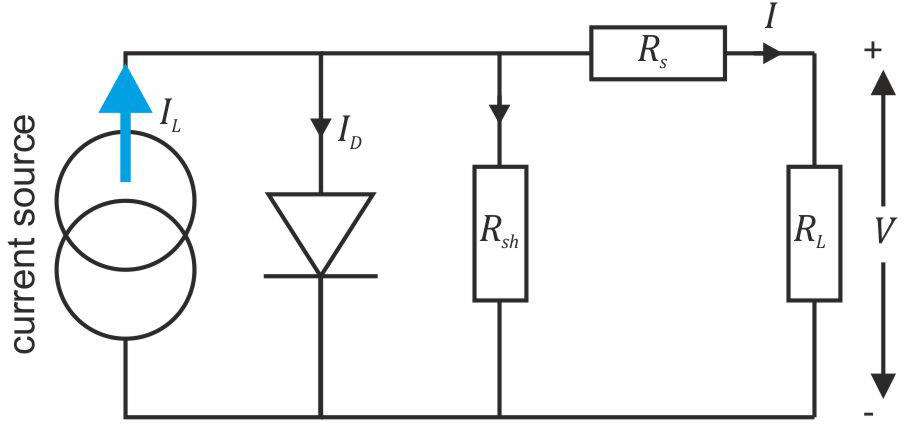
\includegraphics[width=0.9\columnwidth]{model}
	\caption{Solar cell modelling (adapted from \ref{ref:SABPV3})}
	\label{fig:model}
\end{Figure}

The equipment used in this exercise was a \SI{1}{\square\centi\metre} crystalline silicon solar cell with Peltier system for temperature control, a halogen bulb as light source with power density of approximately \SI{0.3}{\kilo\watt\per\square\metre} at a distance of \SI{15}{\centi\metre}, mounted on a mounting rail that can adjust the distance between light source and solar cell, and angle of incidence to the solar cell.

% Baseline IV data acquisition and analysis
\Heading{Baseline data acquisition and analysis}

The Current-Voltage characteristics of the solar cell in baseline measurement conditions was measured firstly, as a reference for various illumination conditions.
\Par

The baseline measurement conditions was defined to be the lowest temperature, normal incidence and with the distance between light source and the solar cell approximately \SI{10}{\centi\metre} apart.

% Measurement
\SubHeading{Measurement}

The $I$-$V$ measurements were done by connecting a resistance box across output terminals of the solar cell, than measure voltages across the resistance box by using a digital multimeter. Voltage across the output terminals can be easily read directly from the multimeter, while current could be calculated by $I = \frac{V}{R}$ and power $P = VI$.
\Par

By taking measurements at various resistance, output current and power vs. output voltage curves was plotted from collected data as shown by Figure \ref{fig:iv10}.
\begin{Figure}
	\ivplottrend{iv10}
	\caption{\ivcap, in baseline measurement condition}
	\label{fig:iv10}
\end{Figure}

% Extract parameters
\SubHeading{Extract parameters}

A few parameters extracted for analysis the characteristic of the solar cell, relative to Figure \ref{fig:iv10}, which were:
\Par

Open circuit voltage $V_{oc}$, the voltage when load resistance connected across the output terminals became very large, shown by x-intercept on $I$-$V$ curve, was \SI{6.11}{\volt}.
\Par

Short circuit current $I_{sc}$, the current flow through shorted output terminals, shown by y-intercept on $I$-$V$ curve. The peak on $I$-$V$ curve near x-axis was caused by imprecise resistance of the resistance box at low resistance, a measurement shows when setting the resistance box to \SI{1}{\ohm}, it was actually about \SI{2.5}{\ohm} measured by a digital multimeter. Therefore, ignoring first few measurements near x-axis, and following the trend of the curve, $I_{sc}$ was approximately \SI{5.5}{\milli\ampere}.
\Par

Voltage and current when output power was at maximum, $V_{mp}$ and $I_{mp}$. To extract them, the maximum power point need to be found firstly by plotting a Power-Voltage curve. As shown in Figure \ref{fig:iv10}, $V_{mp} \approx \SI{0.467}{\volt}$ and $I_{mp} \approx \SI{51.9}{\milli\ampere}$.
\Par

Fill factor, defined by (\ref{eq:ff}), is a key parameter in evaluating solar cell performance. A higher fill factor means less power dissipated in internal losses. All values required to calculate were already known, the fill factor could be therefore calculated as $FF \approx 0.721$.
\begin{Equation}
	FF = \frac{I_{mp}V_{mp}}{I_{sc}V_{oc}}
	\label{eq:ff}
\end{Equation}

% Power efficiency
\SubHeading{Power efficiency}

Power density of light from lamp related to distance as shown in (\ref{eq:lpint}).
\begin{Equation}
	P_{l} \propto \frac{1}{d^2}
	\label{eq:lpint}
\end{Equation}

From laboratory notes, the surface area of the crystalline silicon solar cell was \SI{1}{\square\centi\metre}, and assuming the halogen bulb has a power density of \SI{0.3}{\kilo\watt\per\square\metre} at a distance of \SI{15}{\centi\metre} apart.
\Par

Therefore, power density of light received by the solar cell was about $P_{in} = 0.3 \times 10^3 \cdot \frac{15^2}{10^2} \cdot (1 \times 10^{-2}) ^2 = \SI{0.0675}{\watt}$.
\Par

Power efficiency was calculated as shown in (\ref{eq:eff}).
\begin{Equation}
	\eta = \frac{P_{max}}{P_{in}} = \frac{V_{mp}I_{mp}}{P_{in}} = \frac{0.467 \times 0.0519}{0.0675} = 35.9\%
	\label{eq:eff}
\end{Equation}

% Conclusion
\SubHeading{Conclusion}

From National Renewable Energy Laboratory, the efficiency of best crystalline Si research-cells was $\sim 25\%$ \ref{ref:NRELeff}, which means the value obtained above was not correct or very inaccurate.
\Par

Some possible source of inaccuracy could be the environmental light exist in the laboratory, higher power density of the halogen bulb than the assumed value, which led to a higher power density of light received by the solar cell than the value used in calculation.

% Variation in intensity
\Heading{Variation in intensity}

\begin{Figure}
	\ivlnplot{ivln}
	\caption{\ivlncap}
	\label{fig:ivln}
\end{Figure}

Several $I$-$V$ curves were measured at different intensities of incident light, by changing the distance between the lamp and the solar cell, as shown in Appendix \ref{apx:plots} Figure \ref{fig:iv5}, \ref{fig:iv15} and \ref{fig:iv20}. $V_{oc}$ and $I_{sc}$ were therefore estimated and plotted on Figure \ref{fig:ivln}.
\Par

The estimated point of \SI{5}{\centi\meter} distance was far away from the trend line from other points, possibly because the solar cell was heated by the bulb at that distance, therefore the data obtained were not at the same condition as others, should be ignored.
\Par

$V_{oc}$ and $I_{sc}$ for more distances were also measured using a digital multimeter directly, as shown in the Figure \ref{fig:ivln}. Ignoring first few points taken at a short distance so that the solar cell might be heated by the bulb, since the trend line was similar to the data estimated from $I$-$V$ curve, the trend line obtained here was used in later calculations.
\Par

% Estimate dark saturation current and the ideality factor
\SubHeading{Estimate dark saturation current and ideality factor}

Equation \ref{eq:scm} models simplified solar cell model, ignoring series and shunt resistance:
\begin{Equation}
	I = I_L - I_0 (e^{\frac{q V}{n k T}} - 1)
	\label{eq:scm}
\end{Equation}

When solar cell was in short circuit condition, the equation (\ref{eq:scm}) now becomes:
\begin{Equation}
	I_{sc} = I_L
	\label{eq:scsc}
\end{Equation}

At open circuit condition:
\begin{Equation}
	I_L = I_{sc} = I_0 (e^{\frac{q V_{oc}}{n k T}} - 1)
	\label{eq:scoc}
\end{Equation}

Since $e^{\frac{q V_{oc}}{n k T}}$ should be a lot greater than $1$, therefore $1$ in the equation could be ignored. By taking natural logs of both sides and rearrange, the equation (\ref{eq:scoc}) now becomes:
\begin{Equation}
	\ln I_{sc} = \frac{q}{n k T} V_{oc} + \ln I_0
	\label{eq:lnisc}
\end{Equation}

Looking at the trend line equation obtained in Figure \ref{fig:ivln} and equation (\ref{eq:lnisc}), following relationships were therefore established:
\begin{Gather}
	\frac{q}{n k T} \approx \pgfmathprintnumber{\lnslope}
	\label{eq:lnslope} \\
	\ln I_0 \approx \pgfmathprintnumber{\lnintercept}
	\label{eq:lnintcp}
\end{Gather}

Using room temperature $T = \SI{300}{\kelvin}$, solve the equations: ideality factor $n \approx 1.01$, dark saturation current $I_0 \approx \SI{4.14e-12}{\ampere}$.

% Obtain series and shunt resistance
\SubHeading{Obtain series and shunt resistance}

Since all data points plotted in Figure \ref{fig:ivln} were all on the trend line, so the method of use gradient change at high and low light intensities to estimate series and shunt resistances would not work. Therefore these resistances were estimated using the gradient near $I_sc$ and $V_oc$ on 10cm distance $I$-$V$ curve, as shown in Figure \ref{fig:iv10}.
\Par

Equation \ref{eq:ssmodel} models the solar cell including series and shunt resistance, derived from the solar cell model shown in Figure \ref{fig:model}:
\begin{Equation}
	I = I_L - I_0 (e^{\frac{q (V + I R_s)}{n k T}} - 1) - \frac{V + I R_s}{R_{sh}}
	\label{eq:ssmodel}
\end{Equation}

In short circuit condition, since $R_s << R_{sh}$, current flow through $R_s$ assumed to be $I_L = I_{sc}$, while no current flow through $R_{sh}$. Therefore, at data points near $I_{sc}$, the difference between $I$ and $I_{sc}$ could be assumed to be the current flow through shunt resistor, and the voltage could be assumed to be the voltage across shunt resistor as well. Therefore, the gradient of $I$-$V$ curve near $I_{sc}$ should be $\frac{1}{R_{sh}}$, as indicated by Figure \ref{fig:estshunt}.
\begin{Figure}
	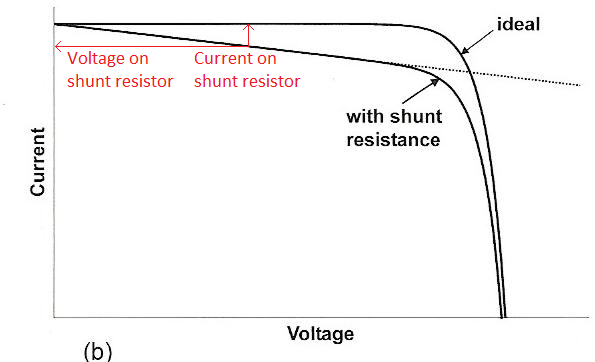
\includegraphics[width=0.9\columnwidth]{estshunt}
	\caption{Estimate shunt resistance (reproduced from \ref{ref:cnote})}
	\label{fig:estshunt}
\end{Figure}

The series resistance can be estimated using the same method, as indicated by Figure \ref{fig:estseries}.
\begin{Figure}
	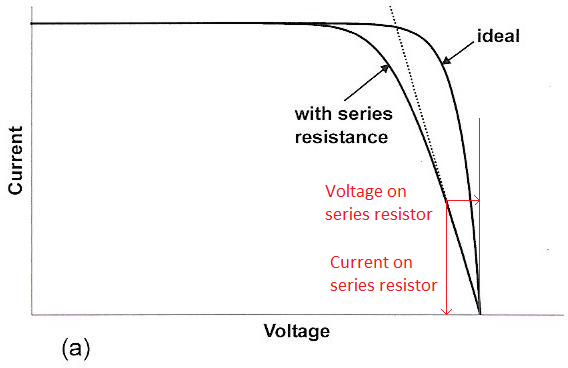
\includegraphics[width=0.9\columnwidth]{estseries}
	\caption{Estimate series resistance (reproduced from \ref{ref:cnote})}
	\label{fig:estseries}
\end{Figure}

Applying the methods described above, from $I$-$V$ curve at \SI{10}{\centi\metre} distance shown by Figure \ref{fig:iv10}, series and shunt resistance therefore estimated as:
\begin{Gather}
	R_{sh} = \frac{-1}{slope_{sc}} \approx \frac{-1}{\pgfmathprintnumber{\slopesc}} \approx \SI{158.5}{\ohm}
	\label{eq:rsh} \\
	R_s = \frac{-1}{slope_{oc}} \approx \frac{-1}{\pgfmathprintnumber{\slopeoc}} \approx \SI{1.41}{\ohm}
	\label{eq:rs}
\end{Gather}

Series and shunt resistance determines fill factor, a power efficient solar cell should have small series resistance and large shunt resistance.

% Variation in angle of incidence
\Heading{Variation in angle of incidence}

Several $I$-$V$ curves were measured at different angle of incidence to the solar cell, as shown in Appendix \ref{apx:plots} Figure \ref{fig:iv10_10}, \ref{fig:iv10_20} and \ref{fig:iv10_30}. Figure \ref{fig:ivangles} shows all plots on the same graph.
\begin{Figure}
	\ivplotangles
	\caption{\ivlncap}
	\label{fig:ivangles}
\end{Figure}

It could be seen from the figure that the maximum output power of the solar cell reduced while angle of incidence increasing, suggests the solar cell could only absorb light from a limited angle of incidence.

% Practical deployment and operation
\Heading{Practical deployment and operation}

The best location for installation of solar cell would be place that can receive most sun light, and the weather condition need to be taken into consideration as well.
\Par

Since Earth are rotating and also orbits the Sun, angle of light coming from the Sun to the solar cell would be varying every day and seasons. Therefore, for maximum power output, the solar cell need to track the Sun, possibly installed on a controllable base and controlled by a computer system.
\Par

The solar cell could also encapsulated in a case or by another coating layer, so that enables it to absorb light from a greater angle of incidence, by changing the angle of light from outside, improves the power efficiency.

\iffalse
% ****************************************** COMMENTS ******************************************
\sepTable
\begin{table}[H]
\caption{Touchscreen interfacing (adapted from \ref{ref:tsNXP})}
\label{tb:ts}
\begin{tabular}{p{0.15\columnwidth} p{0.2\columnwidth} p{0.1\columnwidth} p{0.1\columnwidth} p{0.1\columnwidth}}
	\hline
	Function	& X+	& Y+	& X-	& Y- \\ \hline
	Detection	& Digital input with pull-up	& Open	& Open	& $V_{SS}$ \\ \hline
	Read X	& $V_{CC}$	& ADC1	& $V_{SS}$	& Open \\ \hline
	Read Y	& ADC2	& $V_{CC}$	& Open	& $V_{SS}$ \\ \hline
\end{tabular}
\end{table}
\sepFigure

\begin{figure}[H]
	\centering
	\begin{subfigure}[b]{0.4\columnwidth}
		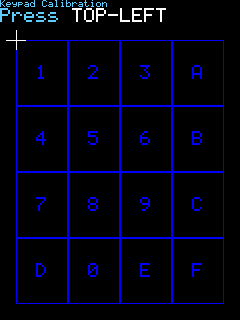
\includegraphics[width=\textwidth]{cap_kp_cal}
		\caption{Keypad calibration}
		\label{fig:capKPCAL}
	\end{subfigure}
	\begin{subfigure}[b]{0.4\columnwidth}
		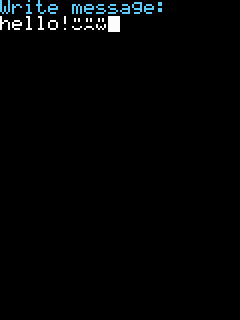
\includegraphics[width=\textwidth]{cap_text}
		\caption{Message writing}
		\label{fig:capText}
	\end{subfigure}
	\caption{Text input GUI}
	\label{fig:capTextInput}
\end{figure}

\begin{enumerate}[label={\arabic*)},align=left,leftmargin=0.5cm,labelwidth=!,topsep=0pt,partopsep=0pt,parsep=0pt,itemsep=0pt]
\item Command (1 byte), the required operation. Commands without COM\_DATA macro does not have data, length byte would not transmitted as well.
\item Length (1 byte).
\item Data (Maximum 64 bytes).
\end{enumerate}
% ****************************************** COMMENTS ******************************************
\fi

% Reference
\begin{Reference}
\item\label{ref:SABPV3}
	\REFOnline{Stuart Boden}{Photovoltaics 3} \url{https://secure.ecs.soton.ac.uk/notes_so/elec2201/STUART%20BODEN%20LECTURES/PV%20LECTURES/ELEC2201_SABSlides_Lecture3_Handout.pdf}
\item\label{ref:cnote}
	\REFOnline{ELEC2201}{Complete Notes} \url{https://secure.ecs.soton.ac.uk/notes_so/elec2201/SECOND%20YEAR%20ELEC2201%20COURSE%20NOTES/Complete%20Notes.pdf}
\item\label{ref:NRELeff}
	\REFOnline{NREL}{Best Research-Cell Efficiencies} \url{http://www.nrel.gov/ncpv/images/efficiency_chart.jpg}
\end{Reference}

\end{Content}

% Appendix. Plots
\newpage
\Appendix{apx:plots}{Additional plots}

\begin{Content}
\begin{Figure}
	\ivplot{iv5}
	\caption{\ivcapapart{5}}
	\label{fig:iv5}
\end{Figure}

\begin{Figure}
	\ivplot{iv15}
	\caption{\ivcapapart{15}}
	\label{fig:iv15}
\end{Figure}

\begin{Figure}
	\ivplot{iv20}
	\caption{\ivcapapart{20}}
	\label{fig:iv20}
\end{Figure}

\begin{Figure}
	\ivplot{iv10_10}
	\caption{\ivcapangle{10}}
	\label{fig:iv10_10}
\end{Figure}

\begin{Figure}
	\ivplot{iv10_20}
	\caption{\ivcapangle{20}}
	\label{fig:iv10_20}
\end{Figure}

\begin{Figure}
	\ivplot{iv10_30}
	\caption{\ivcapangle{30}}
	\label{fig:iv10_30}
\end{Figure}
\end{Content}

\iffalse
\begin{Figure}
	\ivplotall
	\caption{ALL}
	\label{fig:ivall}
\end{Figure}
\fi

\end{document}
